\documentclass[12pt,letterpaper]{article}

\usepackage[utf8]{inputenc}
\usepackage{ragged2e}
\usepackage{amsfonts}
\usepackage{amssymb}
\usepackage{graphicx}
\usepackage{multicol}
\usepackage{changepage}
\usepackage{float}
\usepackage{cite}
\usepackage{url}
\usepackage[left=2.50cm, right=2.50cm]{geometry}
\usepackage[spanish]{babel}
\graphicspath{ {images/} }


\author{Ram\'irez Fuentes Edgar Alejandro}
\title{Entrega 2}
\date {2020-11-03}

\begin{document}
	%encabezado 
	\pagestyle{plain}
	{
		% Imágenes de la portada
		{
			\begin{tabular}
				{
					p{0.75\textwidth} 
					p{0.25\textwidth} 
				}
				
\includegraphics[width=1.5cm, height=2.5cm]{ipn.png} &  
				
\includegraphics[width=2.5cm, height=2cm]{escom.png}
			\end{tabular}
		}
		% Datos de la caratula
		\begin{center}
			\par\vspace{1cm} %Espacio dejado antes del encabezado
			{
				\Huge\textbf
				{
					Instituto Polit\'ecnico Nacional 
					\\[.2cm]Escuela Superior de C\'omputo
				}
			}
			\par\vspace{0.5cm}
			{
				\Large\textbf
				{
					Ingenier\'ia en sistemas computacionales 
					\\[.5cm]An\'alisis y diseño orientado a objetos
				}
			}
			\vfill
			\par\vspace{0.5cm}
			{
				\Large\textbf
				{
					Entrega 2 \\
					CEDAE (Centro de dematológico de alta especialidad)
				}
			}
			\vfill
			\par\vspace{1cm}
			{
				\large\textbf
				{
                    Equipo 3:
                    \\Angeles Hernández Jesús Eduardo
                    \\Chanes Nuñez Ricardo Jehonadab
                    \\García Gamiño Rafael Julian
                    \\Hernández Ceciliano Luis Ángel
                    \\Mendoza Cuellar José Oscar
                    \\Olvera Olvera Kevin Jesús
                    \\Paniagua Juárez Nadia Patricia
                    \\Ramírez Fuentes Edgar Alejandro
                    \\Zamorano Cruz Juan Raymundo
					\\2CV9
				} 
			}
			\par\vspace{3cm}
		\end{center}
		\clearpage
	}
	\newpage
	\pagestyle{plain}
	{
		\begin{center}
			\par\vspace{0.5cm}
			{
				\Huge\textbf
				{
					\'Indice
				}
			}
		\end{center}
					\begin{itemize}
						\item Organización del SCRUM Team ... 3
                        \begin{itemize}
                            \item Product Owner
                            \item SCRUM Master
                            \item Development team
                        \end{itemize}
						\item Acuerdos del SCRUM Team ... 4
						\item Descripción del proyecto ... 5
						\item Requerimientos del proyecto ... 6
                            \begin{itemize}
                                \item Funcionales
                                \item No funcionales
                            \end{itemize}
                        \item Casos de uso ... 8
                        \item Diagramas de casos de uso ... 9
					\end{itemize}
			\vfill
	}
	\newpage
	\pagestyle{plain}
	{
		\par\vspace{0cm}
		{
			\begin{center}
					\Huge\textbf
					{
						Organización del SCRUM Team
					}
			\end{center}
        }
        \par\vspace{0cm}
		{
			\normalsize\textbf
			{
				\justify
                Después de una reunión enfocada a la selección de los roles
                que tendrá cada integrante del equipo, se llegó a la siguiente
                organización.
                \\\\
                \begin{itemize}
                    \item Product Owner - M.C. Maldonado Castillo Idalia 
                    \item SCRUM Master - Hernández Ceciliano Luis Ángel 
                    \item Development team
                        \begin{itemize}
                            \item Equipo de análisis
                                \begin{itemize}
                                    \item Angeles Hernández Jesús Eduardo
                                    \item Hernández Ceciliano Luis Ángel
                                \end{itemize}
                            \item Equipo de diseño
                            \begin{itemize}
                                \item Panigua Juárez Nadia Patricia
                                \item Zamorano Cruz Juan Raymundo
                            \end{itemize}
                            \item Equipo de desarrollo
                            \begin{itemize}
                                \item Bases de Datos
                                    \begin{itemize}
                                        \item Mendoza Cuellar José Oscar
                                        \item Olvera Olvera Kevin Jesús
                                    \end{itemize}
                                \item Front-end
                                \begin{itemize}
                                    \item Ramírez Fuentes Edgar Alejandro
                                    \item Panigua Juárez Nadia Patricia
                                    \item Zamorano Cruz Juan Raymundo
                                \end{itemize}
                                \item Back-end
                                \begin{itemize}
                                    \item Chanes Nuñez Ricardo Jehonadab
                                    \item García Garmiño Rafael Julian
                                    \item Ramírez Fuentes Edgar Alejandro
                                \end{itemize}
                            \end{itemize}
                        \end{itemize}
                \end{itemize}
            }
        }
    }
    \newpage
	\pagestyle{plain}
	{
		\par\vspace{0cm}
		{
			\begin{center}

					\Huge\textbf
					{
						Acuerdos del SCRUM Team
					}
			\end{center}
        }
        \par\vspace{0cm}
		{
			\normalsize\textbf
			{
                \justify
                En una de las reuniones diarias del SCRUM se llegaron a
                los siguientes acuerdos, los cuales deberán ser cumplidos de 
                manera exacta.
                \begin{itemize}
                    \item Daily standup meetings
                    \begin{itemize}
                        \item Las daily meeting se realizarán de Lunes a Viernes en un horario de 22:00 a 22:18 
                        \item Cada participante tendrá 2 minutos para hablar
                        \item Cada integrante deberá tener listos los puntos a tratar antes de la reunión para evitar prolongar la reunión
                        \item No se tendrá tolerancia ante retardos
                        \item Si un integrante tiene más de cinco faltas en estas reuniones, se expulsará del equipo por falta de compromiso con el proyecto
                        \item Solo se tocarán temas con respecto a actividades realizadas el día de la reunión y obstáculos que se tienen para la realización de futuras actividades
                        \item Si los equipos desean reunirse por su parte para tratar dudas acerca del proyecto, son libres de hacerlo.
                    \end{itemize}
                    \item Sprint planning meetings, Sprint review meeting y Sprint retrospective meeting
                    \begin{itemize}
                        \item Este tipo de reuniones se realizarán en los días sabádos a las 22:00 para la dedicación de tiempo necesario.
                        \item No habrá tolerancia ante retrasos en este tipo de reuniones
                        \item No habrá tolerancia ante ausencia en este tipo de reunión. Si algún integrante llega a faltar, se pondrá a votación su estancia en el equipo de trabajo 
                        \item La duración de la reunión será dependiente del entendimiento organización, opiniones del equipo acerca del proyecto 
                    \end{itemize}
                \end{itemize}
            }
        }
    }
    \newpage
	\pagestyle{plain}
	{
		\par\vspace{0cm}
		{
			\begin{center}
					\Huge\textbf
					{
						Descripción del proyecto
					}
			\end{center}
        }
        \par\vspace{0cm}
		{
			\normalsize\textbf
			{
                \justify
                Se desarrollará un sistema web el cual apoyará a la clínica CEDAE a la gestión de doctores titulares,
                doctores auxiliares, trabajadores de la clínica, pacientes, stock de medicina, citas médicas, expedientes médicos,
                recetas médicas, entre otras futuras funcionalidades.
                Además, se implementarán todos aquellos servicios y subservicios que la clínica CEDAE presta para así lograr satisfacer
                las necesidades del cliente.
                \\\\
                El sistema le permitirá al médico titular visualizar expedientes de sus pacientes, emitir recetas tanto físicas,
                por correo electrónico o por la plataforma web, permitir el acceso a su receta médica de sus pacientes, entre otras futuras funcionalidades.
                \\\\
                El sistema permitirá a los usuarios, únicamente aquellos registrados en la plataforma, visualizar recetas previamente autorizadas por 
                su médico, visualizar futuras citas, entre otras futuras funcionalidades.
                \\\\
                Para el módulo del área de farmacia se llevará el control de los medicamentos en stock, se dará alerta de aquellos medicamentos que estén cerca de incumplimiento 
                de normas de COFEPRIS para así ayudar al cliente a priorizar la venta de medicamento cercano a ser desechado, entre otras futuras funcionalidades.
                \\\\
                Por parte del sector administrativo de la clínica permitirá generar citas, generar reportes estadísticos que el cliente requiera, entre futuras funcionalidades.
                \\\\
                Nota: La descripción actual del proyecto es con base en la información que hasta el momento se tiene acerca del proyecto.
            }
        }
    }
    \newpage
	\pagestyle{plain}
	{
		\par\vspace{0cm}
		{
			\begin{center}
					\Huge\textbf
					{
						Requerimientos del proyecto
					}
			\end{center}
		}
		\par\vspace{0cm}
		{
			\normalsize\textbf
			{
                \justify
                \begin{itemize}
                    \item Requerimientos funcionales
                    \begin{enumerate}
                        \item El sistema permitirá a cada usuario iniciar y cerrar sesión en el sistema.
                        \item El sistema permitirá al usuario administrador registrar otros usuarios.
                        \item El sistema permitirá al usuario administrador dar de baja a otros usuarios.
                        \item El sistema permitirá al usuario administrador modificar la información de otros usuarios.
                        \item El sistema permitirá al usuario recepcionista agendar citas para pacientes.
                        \item El sistema permitirá al paciente consultar las fechas de sus citas a través de su cuenta.
                        \item El sistema permitirá al médico titular generar recetas médicas.
                        \item El sistema permitirá al médico titular generar o hacer cambios al expediente clínico de pacientes.
                        \item El sistema permitirá a los médicos titulares y auxiliares consultar expedientes clínicos de sus pacientes.
                        \item El sistema permitirá al paciente consultar su expediente clínico a través de su cuenta.
                        \item El sistema permitirá al médico titular habilitar los expedientes clínicos para su consulta por parte del usuario.
                        \item El sistema permitirá al usuario administrador generar de reportes estadísticos.
                        \item El sistema contará con manejo de almacén de farmacia.
                        \item El sistema permitirá a los médicos consultar la disponibilidad de medicamentos en farmacia.
                        \item El sistema permitirá al encargado de farmacia consultar la disponibilidad de medicamentos.
                        \item El sistema generará una advertencia para los usuarios encargados de farmacia cuando un medicamento esté pronto a caducar o infringir las normas de COFEPRIS.
                        \item El sistema permitirá a los médicos generar recetas físicas y electrónicas (Vistas en sistema o enviadas por correo electrónico).
                        \item El sistema permitirá llevar un registro del personal que atendió al paciente para cada consulta que este tuvo.
                        \item El sistema permitirá agendar citas a usuarios sin registro.
                        \item \item Las citas solo podrán ser agendadas en el calendario en tiempos de 30 minutos durante el horario de atención.
                        \item La duración de las citas de primera vez será de 1 hora.
                        \item La duración de las citas  subsecuentes será de 30 minutos.
                        \item Cuando se agenda una cita de primera vez en línea, el usuario no podrá escoger el médico que lo atenderá, solo el horario.
                        \item Cuando se agenda una cita de primera vez ya sea de manera presencial o telefónica, ell usuario podrá elegir el médico y el horario de su cita.
                        \item El sistema enviará correos electrónicos para confirmación de las citas.
                        \item El sistema permitirá al usuario recepcionista consultar la agenda de cada médico titular.
                        \item El sistema permitirá al usuario recepcionista ver las citas de todos los usuarios.
                        \item El sistema permitirá al usuario recepcionista realizar cobros de consultas.
                        \item El sistema permitirá al encargado de farmacia realizar cobros por medicamentos.
                        \item El sistema permitirá al encargado de farmacia modificar la existencia de medicamentos en inventario.
                    \end{enumerate}
                    \item Requerimientos no funcionales
                    \begin{enumerate}
                        \item Los expedientes clínicos serán generados con base en la norma NOM-024-SSA3-2010.
                        \item El paciente podrá ver su expediente médico únicamente si ha pedido autorización.
                        \item Las caducidades de medicamentos serán tratadas conforme a las normas de la COFEPRIS.
                        \item El surtido de recetas por parte de la farmacia se debe apegar al Artículo 226 de la Ley General de Salud.
                        \item Se debe de cumplir con la Ley Federal de Protección de Datos Personales en Posesión de los Particulares para los datos almacenados de los usuarios.
                        \item La clínica atenderá en un horario de Lunes a Viernes de 10:00 a 20:00 horas.
                        \item El sistema no permitirá agendar cita con un médico en específico en su horario de comida.
                        \item El sistema será completamente funcional en el navegador Google Chrome en la versión Versión 86.0.4240.183 (Build oficial) o posterior.
                    \end{enumerate}
            \end{itemize}
            Nota: Los siguientes requirimientos están sujetos a cambios, por lo cual no se deberán tomar como requerimientos finales.
			}
		}
	}
    \newpage
	\pagestyle{plain}
	{
		\par\vspace{0cm}
		{
			\begin{center}
					\Huge\textbf
					{
						Casos de uso
					}
			\end{center}
        }
        \par\vspace{0cm}
		{
			\normalsize\textbf
			{
                \justify
                Casos de uso por modulo del sistema
                \newline
                \newline
                Modulo de gestión de usuarios
                \begin{itemize}
                    \item Registrar usuario
                    \item Dar de baja usuario
                    \item Modificar información
                    \item Recuperar cuenta
                    \item Ver usuarios registrados
                    \item Iniciar sesión
                    \item Ver perfil
                    \item Cerrar sesión
                    \item Cambiar contraseña
                    \item Ver paciente
                \end{itemize}
                Modulo de inventario
                \begin{itemize}
                    \item Buscar medicamento
                    \item Agregar medicamento
                    \item Dar de baja medicamento
                    \item Ver inventario
                    \item Notificar stock
                \end{itemize}
            }
        }
    }
    \newpage
	\pagestyle{plain}
	{
		\begin{center}
			\par\vspace{0.5cm}
			{
				\Huge\textbf
				{
					Diagramas de casos de uso
				}
			}
        \end{center}
    \section{Diagramas del modulo de gestión de usuarios}
        \begin{figure}[H]
            \centering
            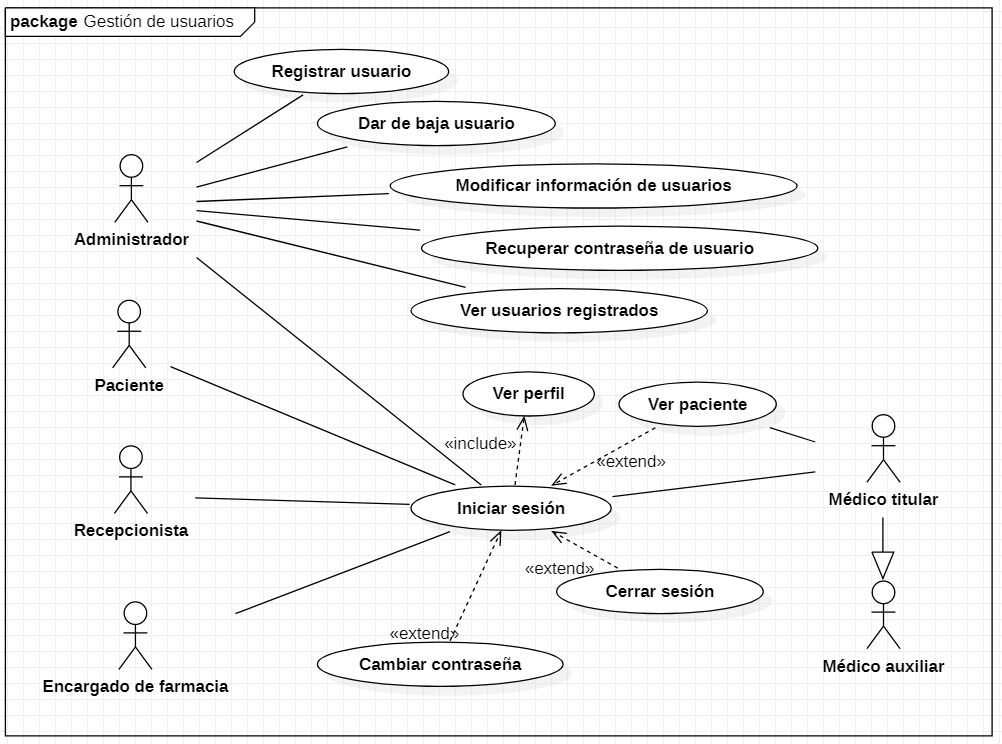
\includegraphics [scale=0.5]{gestionUsuarios}
            \caption{Diagrama de gestión de usuarios}
        \end{figure}
        \begin{figure}[H]
            \centering
            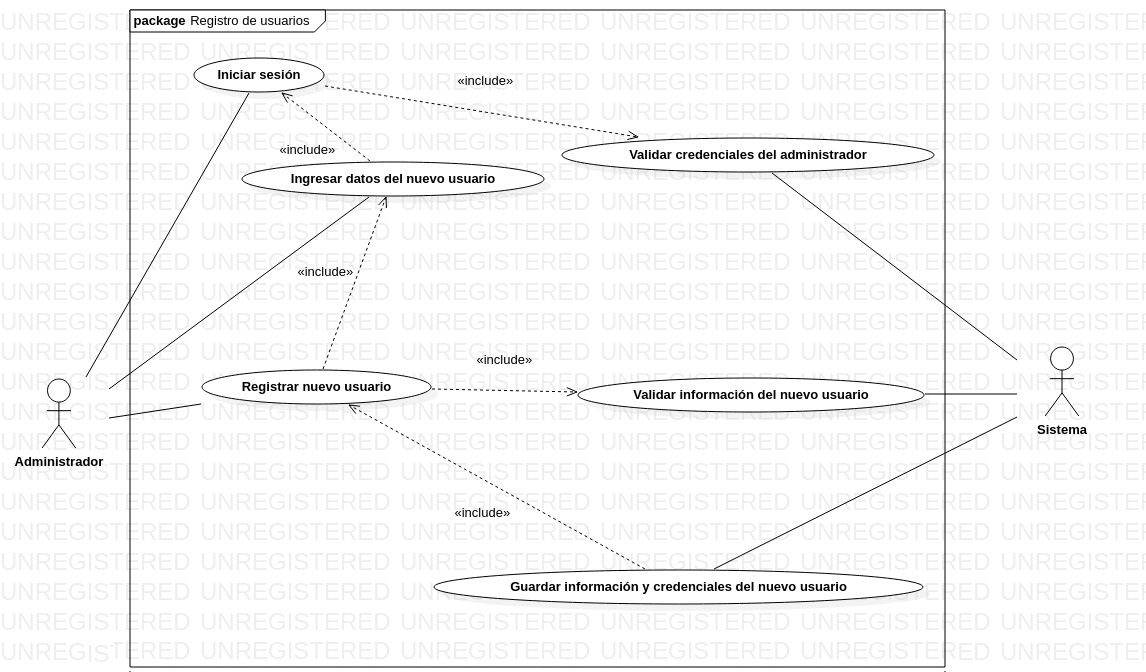
\includegraphics [scale=0.35]{alta_usuarios}
            \caption{Diagrama de registro de usuario}
        \end{figure}
        \begin{figure}[H]
            \centering
            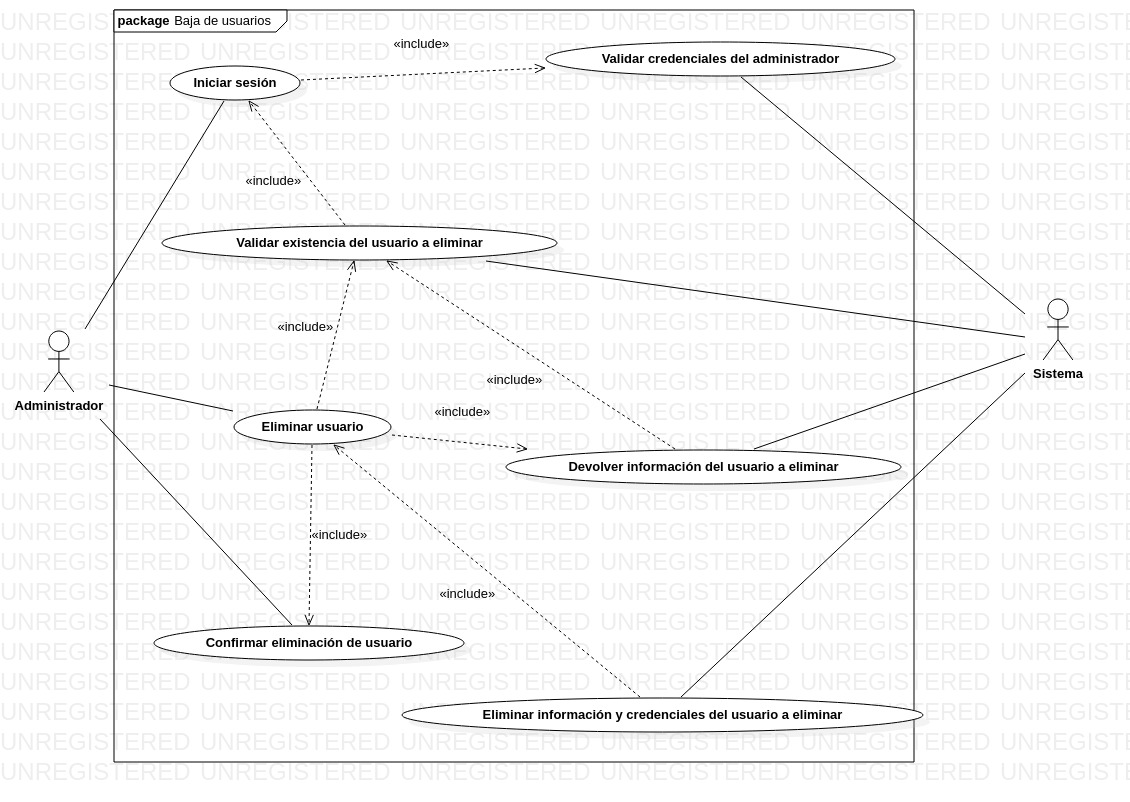
\includegraphics [scale=0.3]{baja_usuarios}
            \caption{Diagrama de baja de usuario}
        \end{figure}
        \begin{figure}[H]
            \centering
            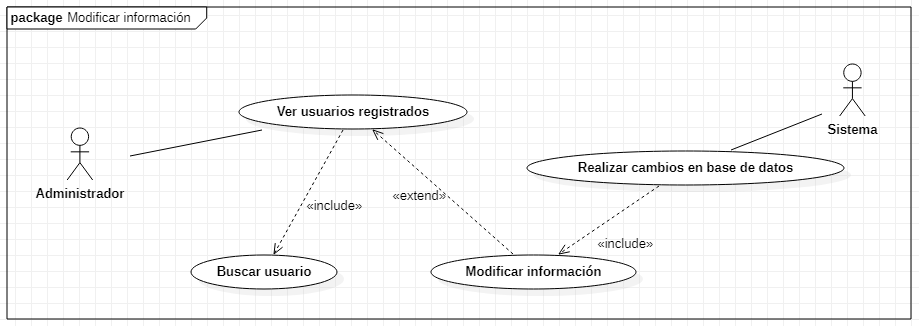
\includegraphics [scale=0.6]{modificarInformacion}
            \caption{Diagrama de modificación de información}
        \end{figure}
        \begin{figure}[H]
            \centering
            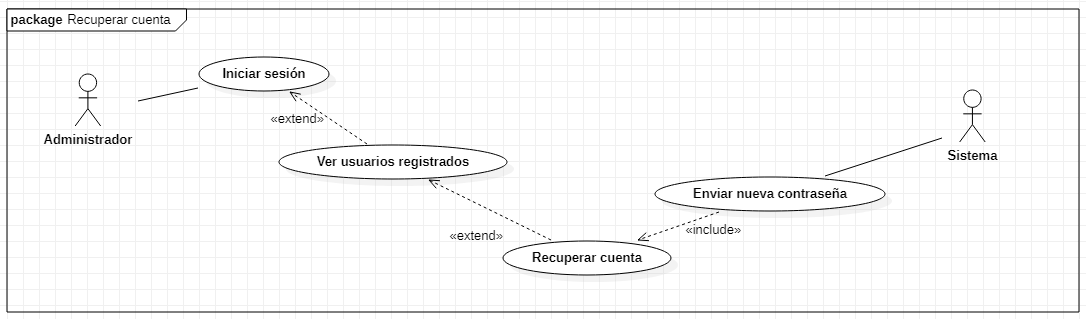
\includegraphics [scale=0.5]{recuperarCuenta}
            \caption{Diagrama de recuperación de cuenta}
        \end{figure}
        \begin{figure}[H]
            \centering
            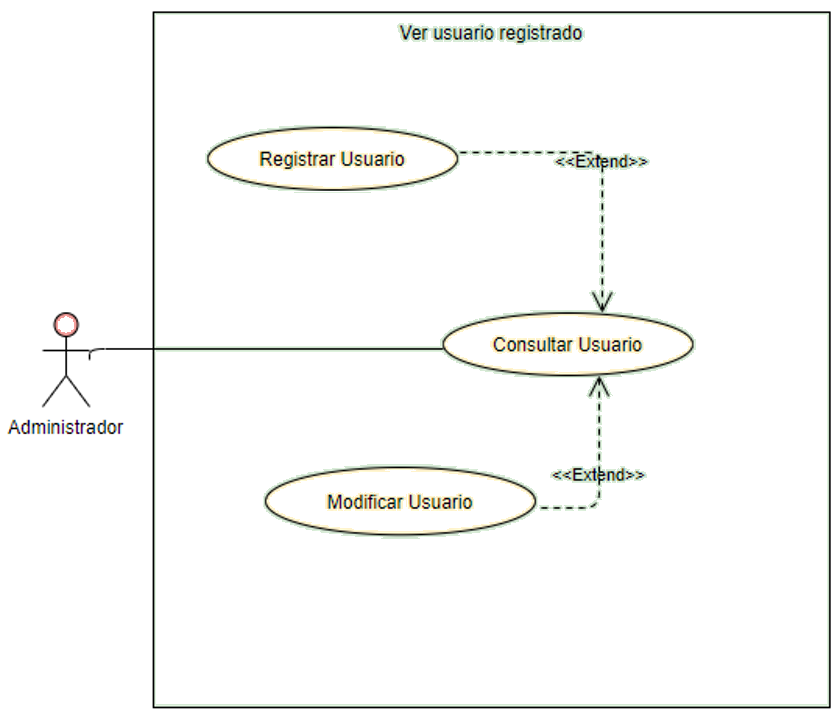
\includegraphics [scale=0.3]{verUsuario}
            \caption{Diagrama de visualización de usuarios}
        \end{figure}
        \begin{figure}[H]
            \centering
            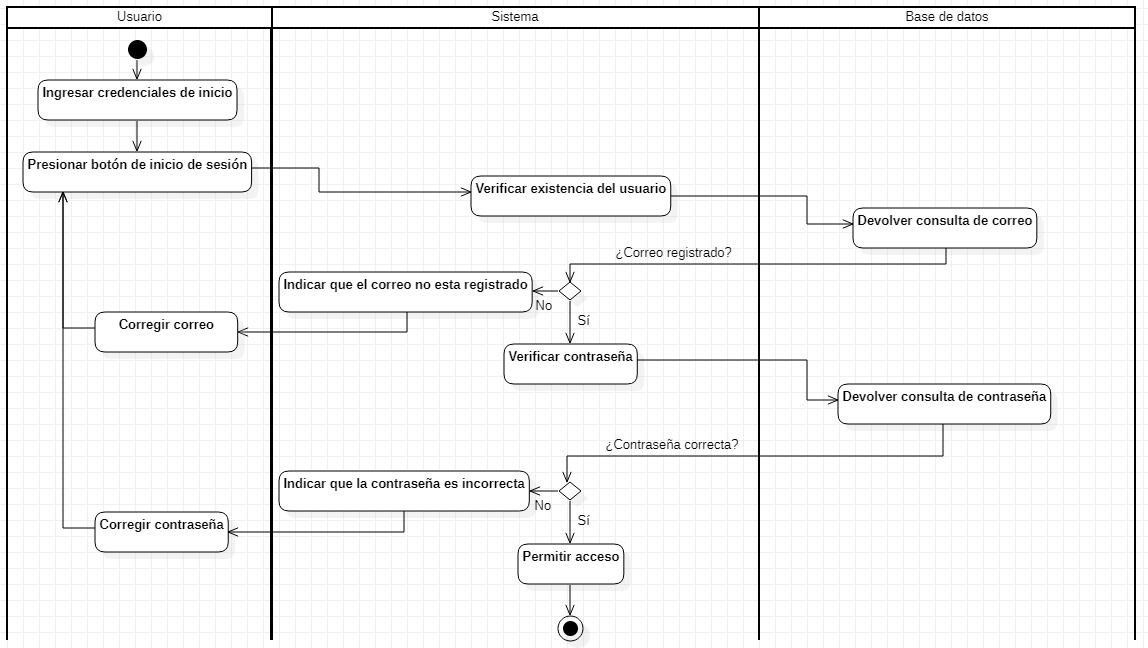
\includegraphics [scale=0.3]{iniciarSesion}
            \caption{Diagrama de inicio de sesión}
        \end{figure}
        \begin{figure}[H]
            \centering
            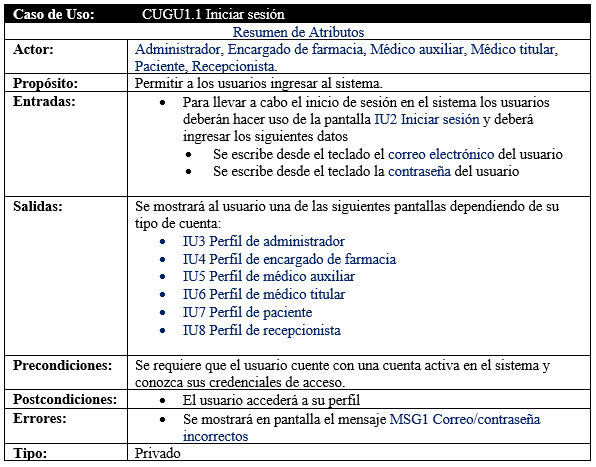
\includegraphics [scale=0.9]{especificacionInicio}
        \end{figure}
        \begin{figure}[H]
            \centering
            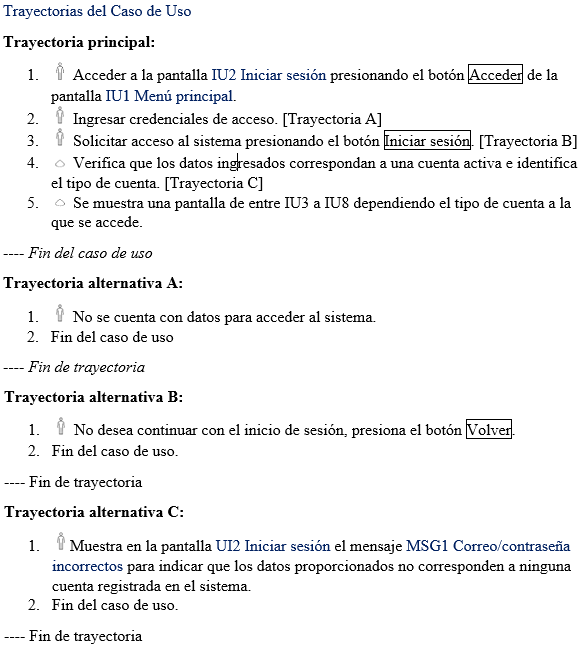
\includegraphics [scale=0.9]{trayectorias}
        \end{figure}
        \begin{figure}[H]
            \centering
            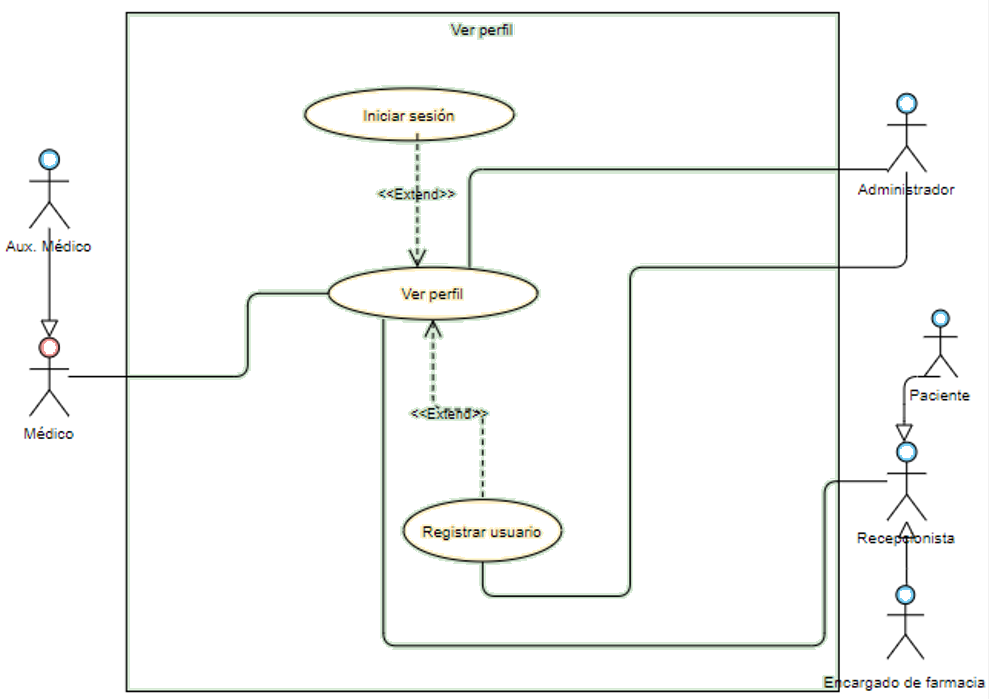
\includegraphics [scale=0.5]{verPerfil}
            \caption{Diagrama de visualización de perfil}
        \end{figure}
        \begin{figure}[H]
            \centering
            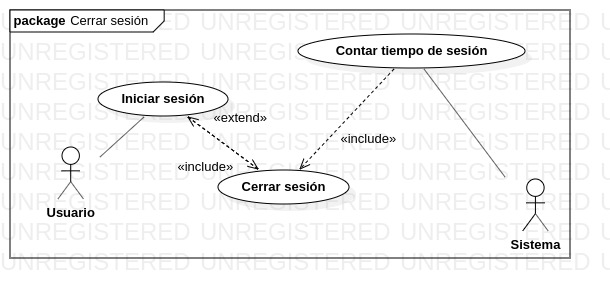
\includegraphics [scale=0.6]{cerrarSesion}
            \caption{Diagrama de cerrar sesión}
        \end{figure}
        \begin{figure}[H]
            \centering
            \includegraphics [scale=0.6]{cambiarContraseña}
            \caption{Diagrama de cambio de contraseña}
        \end{figure}
        \begin{figure}[H]
            \centering
            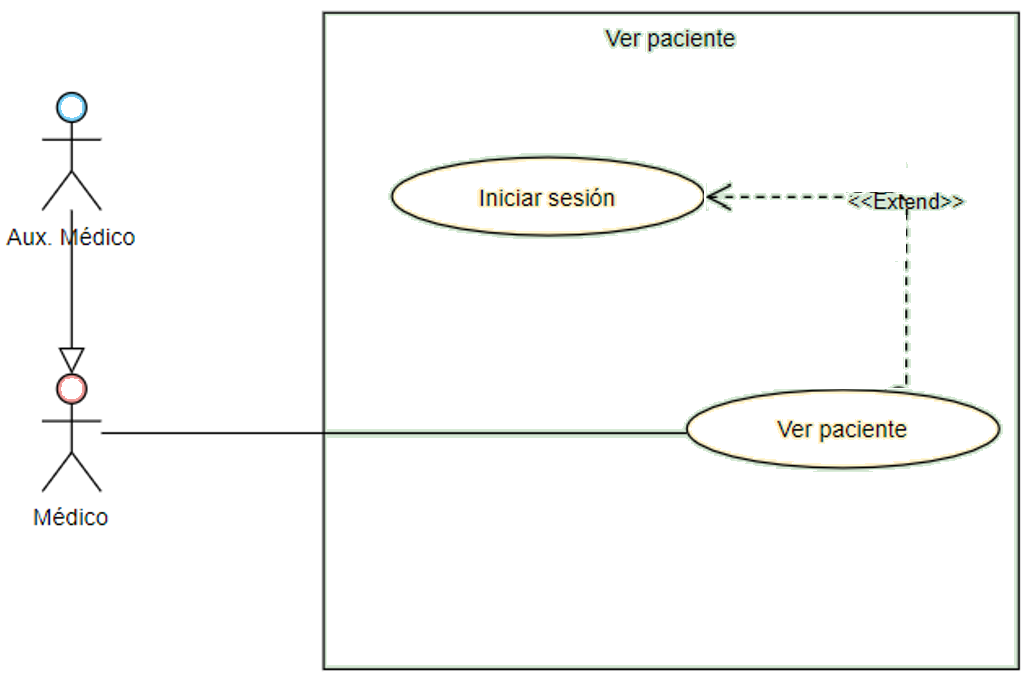
\includegraphics [scale=0.35]{verPaciente}
            \caption{Diagrama de visualización de paciente}
        \end{figure}
        
        \newpage
    \section{Diagramas del modulo de gestión de inventario}
        \begin{figure}[!htb]
            \centering
            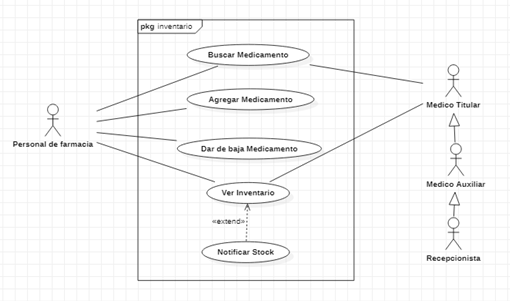
\includegraphics [scale=0.8]{gestionInventario}
            \caption{Diagrama de gestión de inventario}
        \end{figure}
        \begin{figure}[!htb]
            \centering
            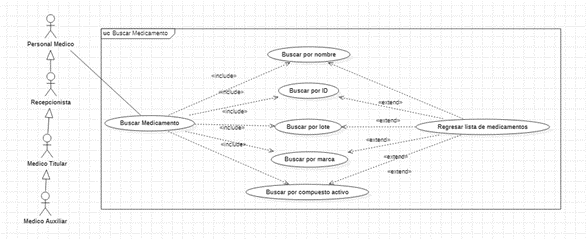
\includegraphics [scale=0.9]{buscarMedicamentos}
            \caption{Diagrama de busqueda de medicamento}
        \end{figure}
        \begin{figure}[!htb]
            \centering
            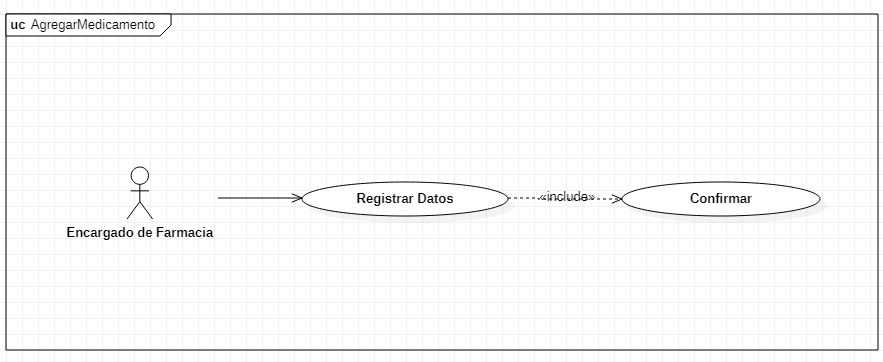
\includegraphics [scale=0.5]{agregarMedicamento}
            \caption{Diagrama de agregar medicamento}
        \end{figure}
        \begin{figure}[!htb]
            \centering
            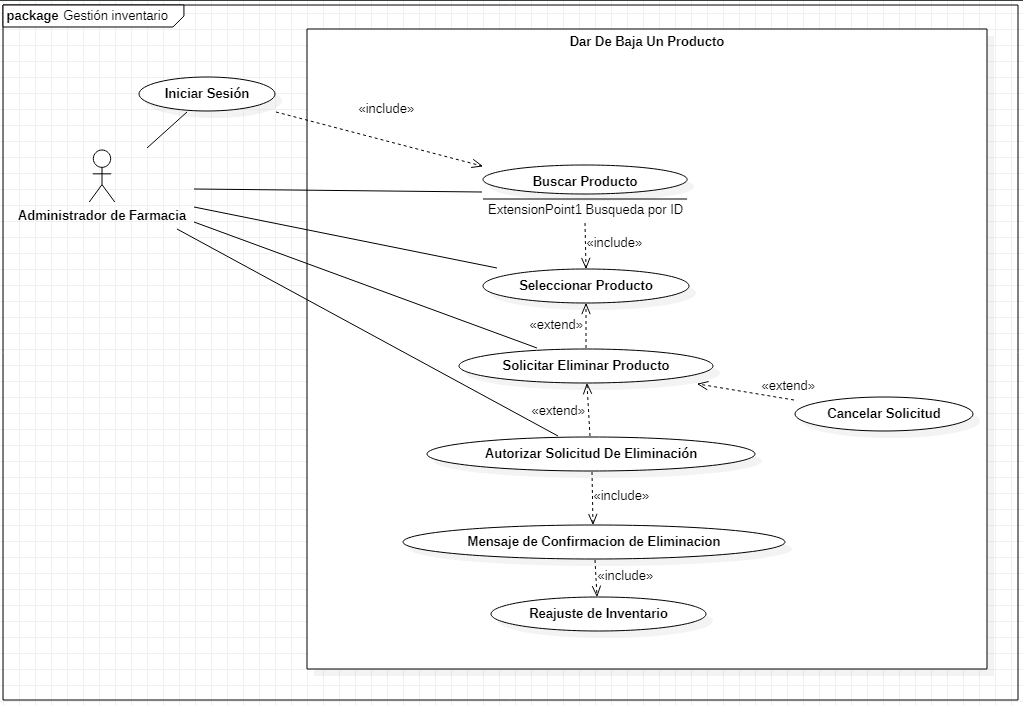
\includegraphics [scale=0.5]{bajaProducto}
            \caption{Diagrama de baja de medicamento}
        \end{figure}
        \begin{figure}[!htb]
            \centering
            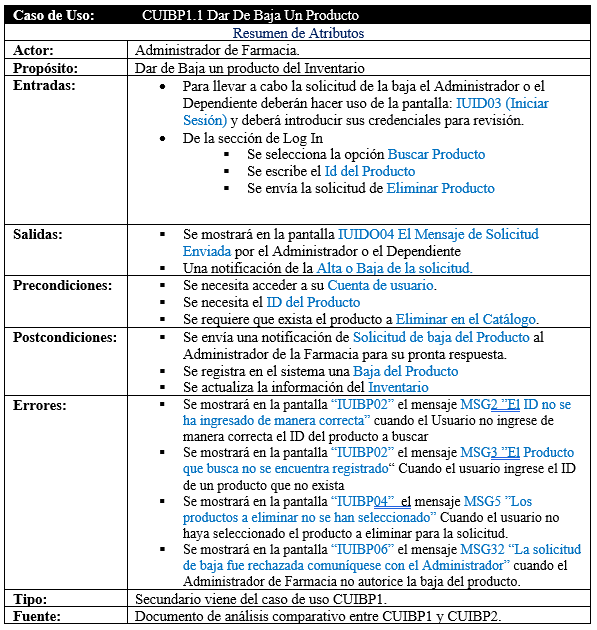
\includegraphics [scale=0.9]{especificacionBajaProducto}
        \end{figure}
        \begin{figure}[!htb]
            \centering
            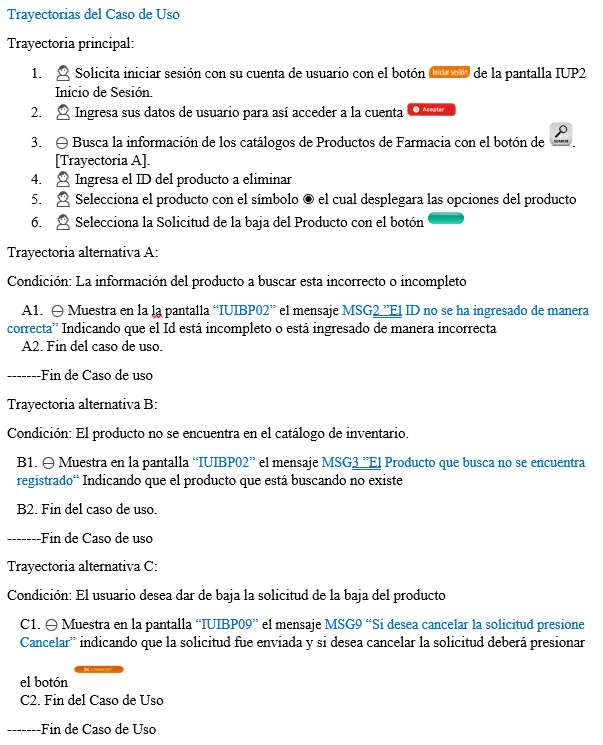
\includegraphics [scale=0.9]{trayectoriaBajaMedicamento}
        \end{figure}
        \begin{figure}[!htb]
            \centering
            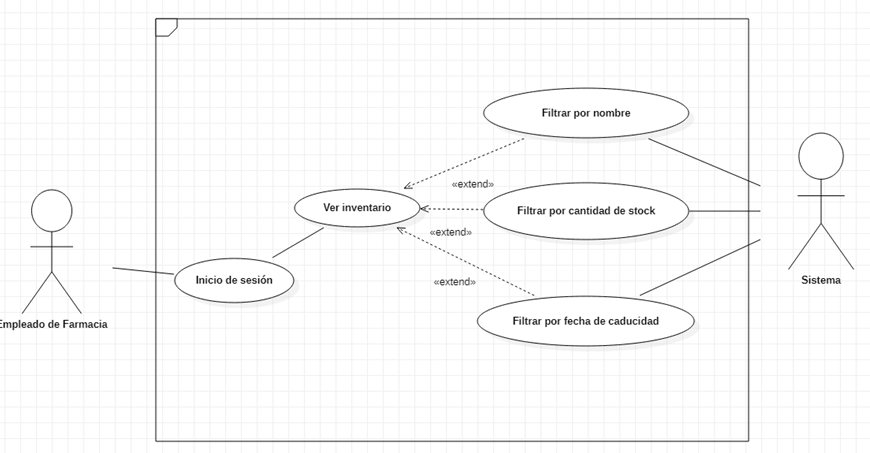
\includegraphics [scale=0.5]{verInventario}
            \caption{Diagrama de visualización de inventario}
        \end{figure}
        \begin{figure}[!htb]
            \centering
            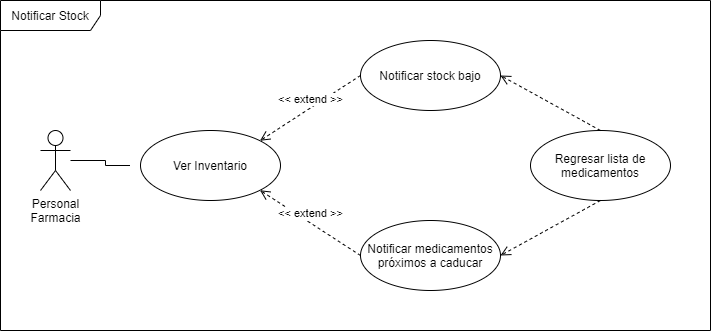
\includegraphics [scale=0.5]{notStock}
            \caption{Diagrama de notificación de stock}
        \end{figure}
			\vfill
	}
\end{document}